\documentclass[12pt]{article}
\usepackage{geometry}
\geometry{a4paper, total={170mm, 250mm}}
\title{\textbf{Homework 5}}
\author{Maedeh Karkhane Yousefi}
\usepackage{float}
\usepackage{graphicx}
\usepackage{amsmath}
\usepackage{subcaption}
\begin{document}
\maketitle
\part*{1. Exercise 4.5: 2D Random Walk}
\paragraph*{} Expanding the direction choices of the previous example gives us the Essentials for this example. I plotted 2 figures by calculating the Radius of Gyration and the squared distance from the first position (0,0).
\begin{figure}[H]
	\centering
	\begin{subfigure}[t]{0.8\textwidth}
		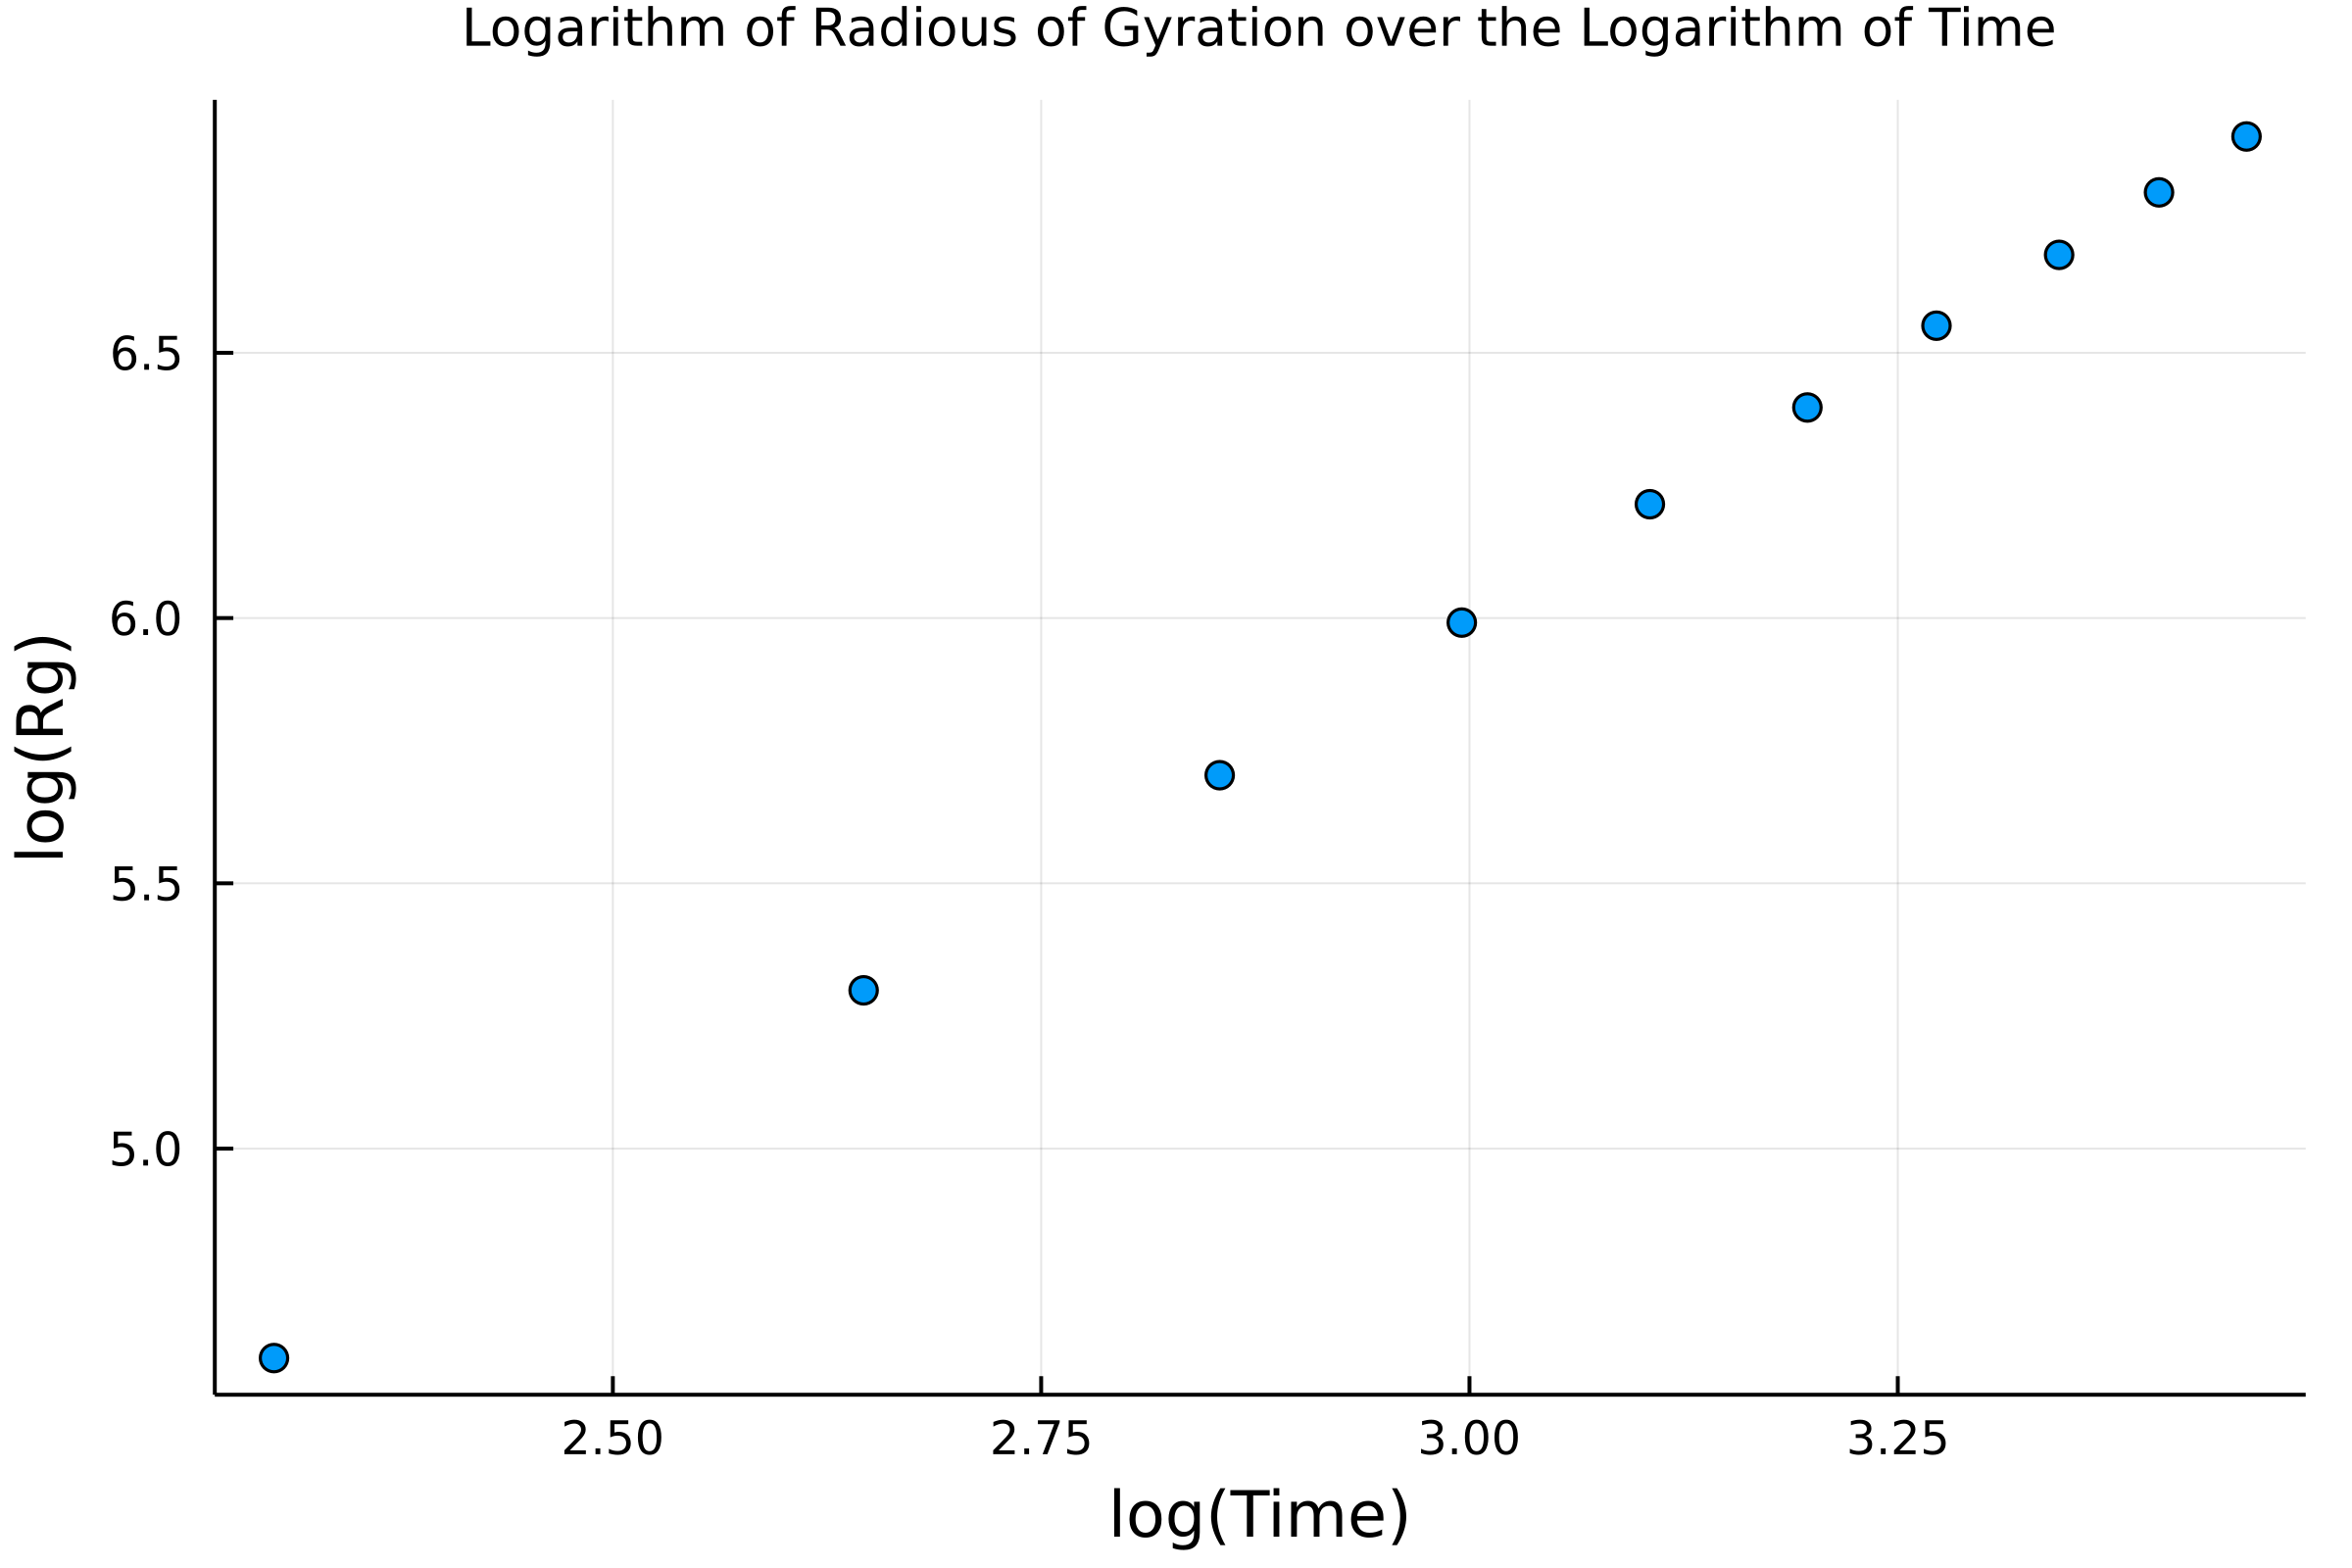
\includegraphics[width=\textwidth]{Rg_Time.png}
		\label{fig:mesh1.1}
		\caption{}
	\end{subfigure}\par\bigskip 
	\begin{subfigure}[t]{0.8\textwidth}
		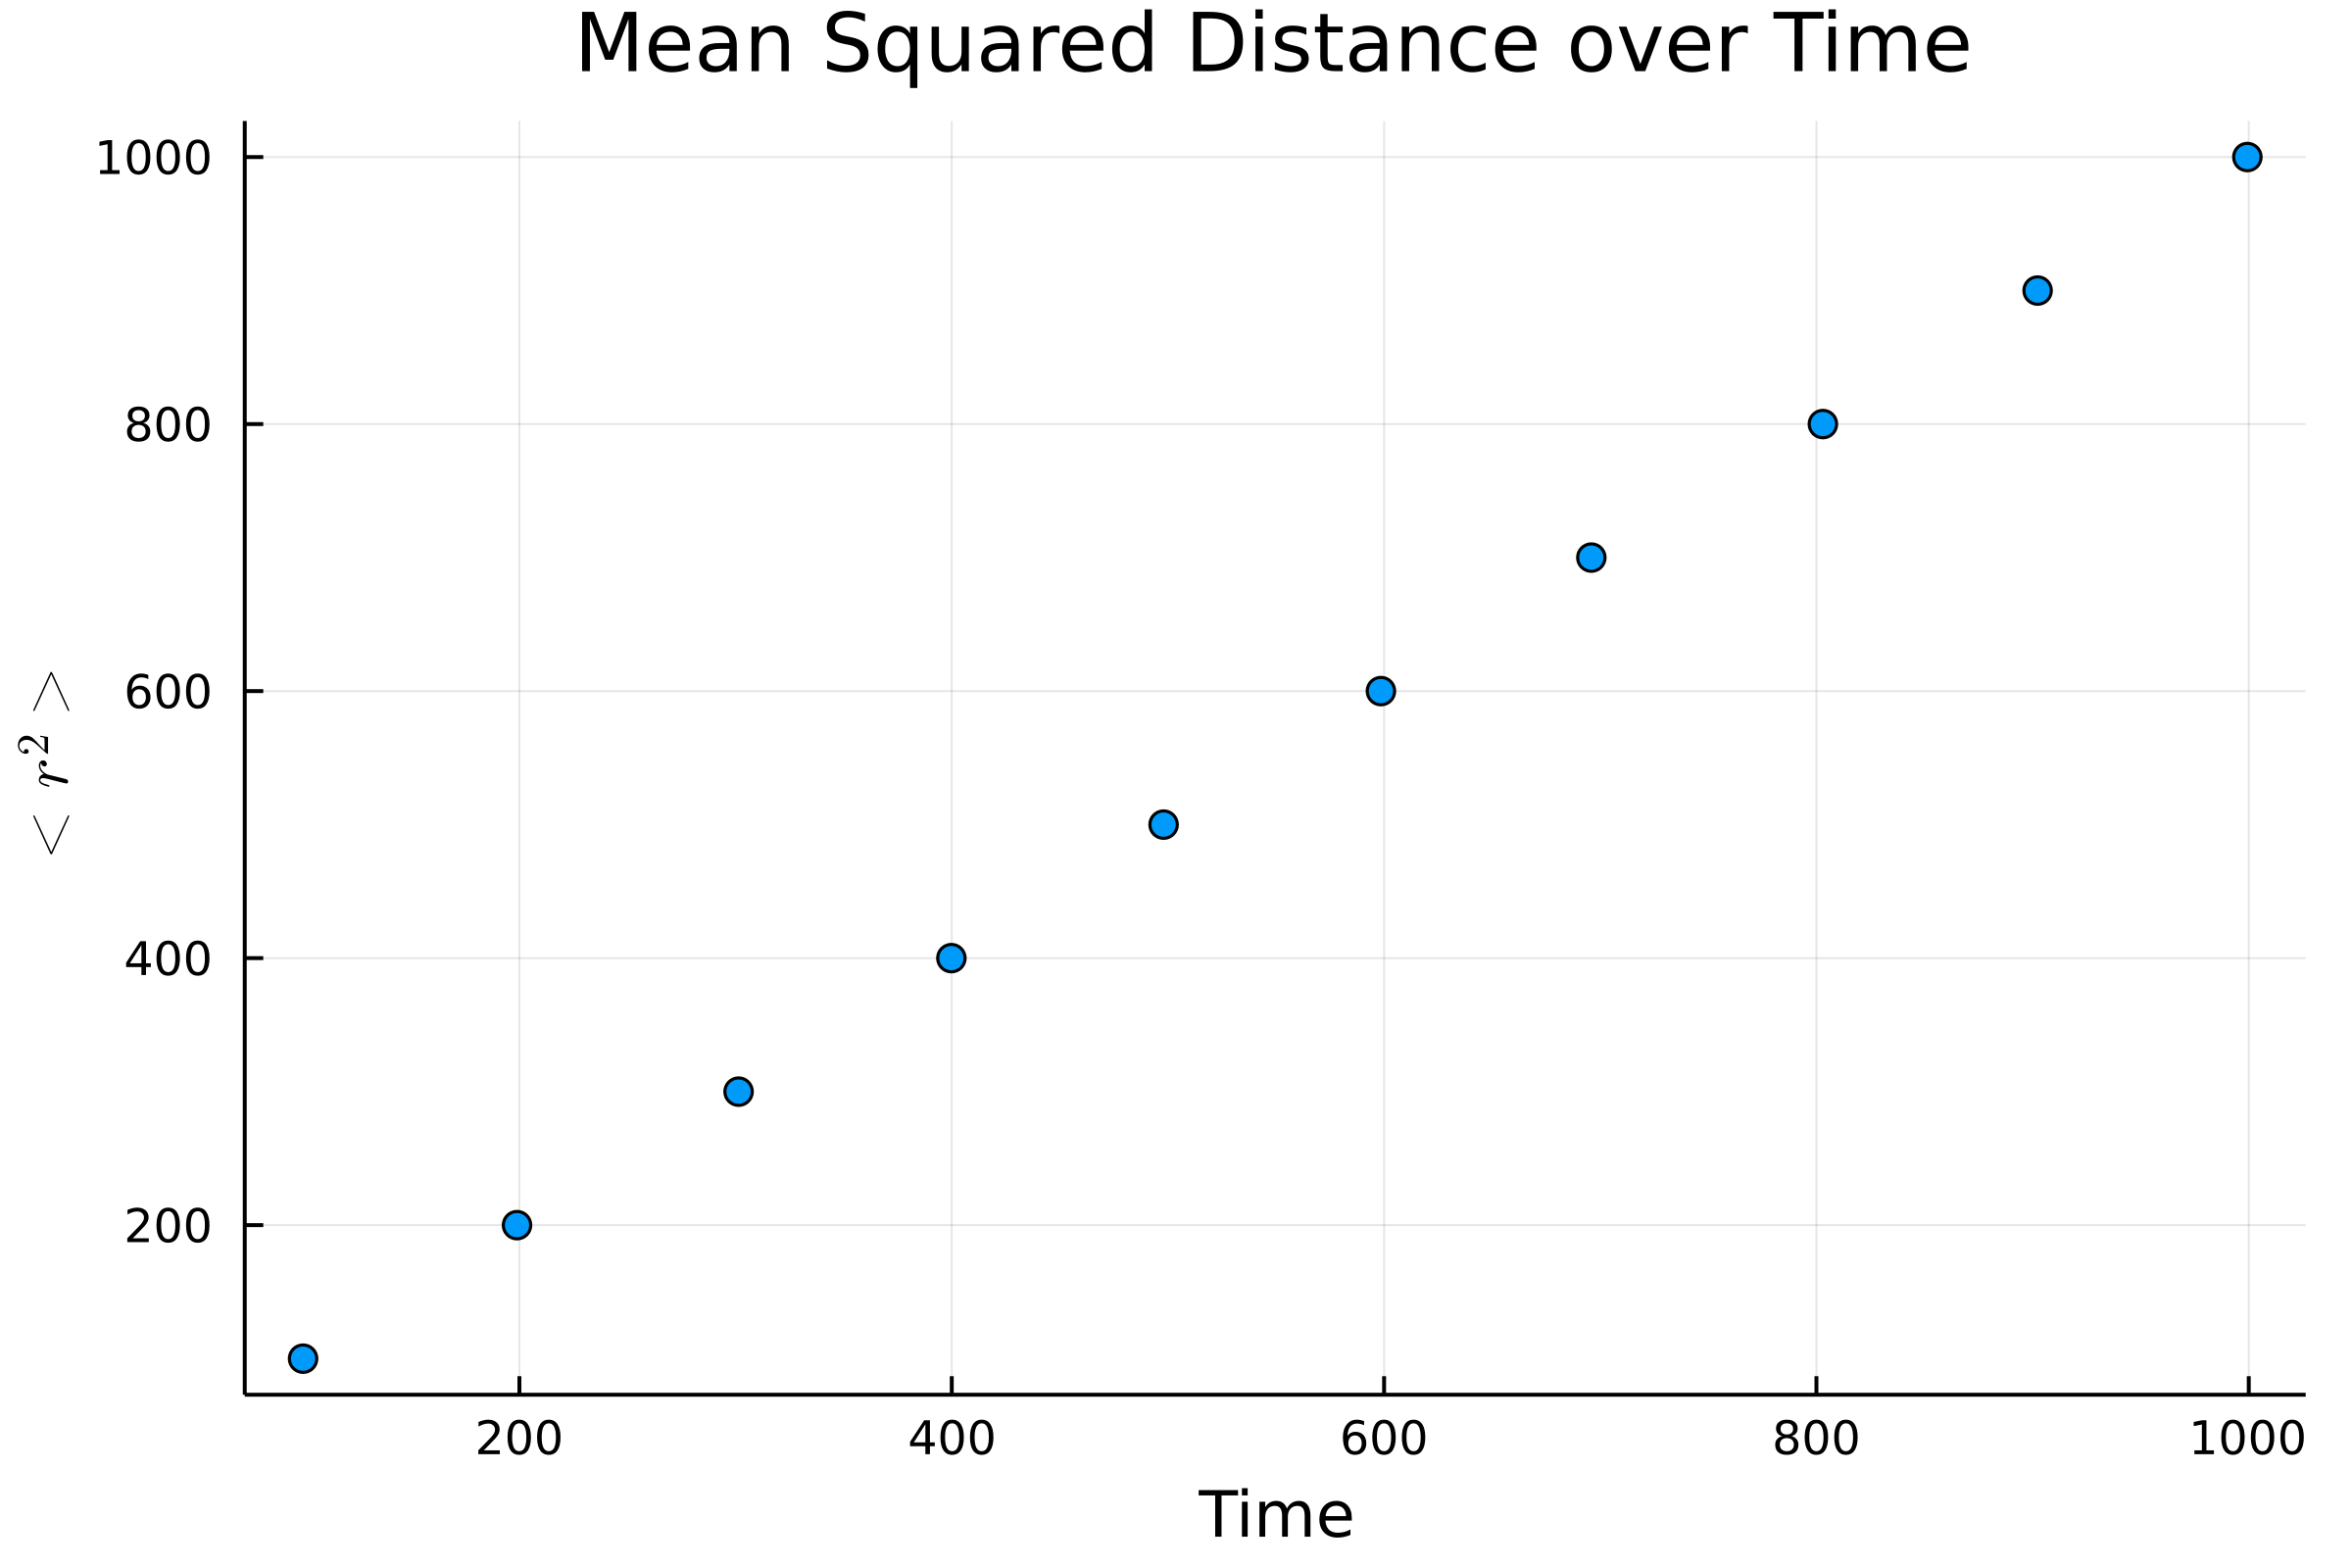
\includegraphics[width=\textwidth]{MeanSquare(r)_Time.png}
		\label{fig:mesh1.2}
		\caption{}
	\end{subfigure}
	\label{fig:mesh1}
	\caption{Figures regarding the confirmation of relations wanted in example 4.5. Which are: $R_{g}=\sqrt{<r^{2}>} \sim t^{\nu}$ and $<r^{2}>=2 d D t$. First position=(0,0), Number of run-times= 100000, }
\end{figure}
\part*{2. Exercise 4.6: Aggressive Layer Deposition}
I set the boundary conditions, get the highest filled place in the network at each step, fill a position after 3 successful deposition( which happens after collision with a filled position). There are two limits which move with the peak of the layer at every step: The lowest, which we choose the random particle from this row of the network, and the top one, which is 5 entries away from the latter and emits every particle that moves beyond this limit. 
\paragraph*{}I tried so hard for the code to work and changed it so much, that I don't know what I'm looking at any more, so I just quit!The code is available though. 
\part*{3. Exercise 4.7: Self-Avoid Random Walk}
\paragraph*{} A simple 2D random walker has $4^{N}$ possible ways to walk around in a network. a self-avoiding random walker, though gives away the choices in order to avoid passing a previous crossed position. I learned to write the algorithm using a rescue function, a function calling itself N times. 
\begin{figure}[H]
	\centering
	\begin{subfigure}[t]{0.8\textwidth}
		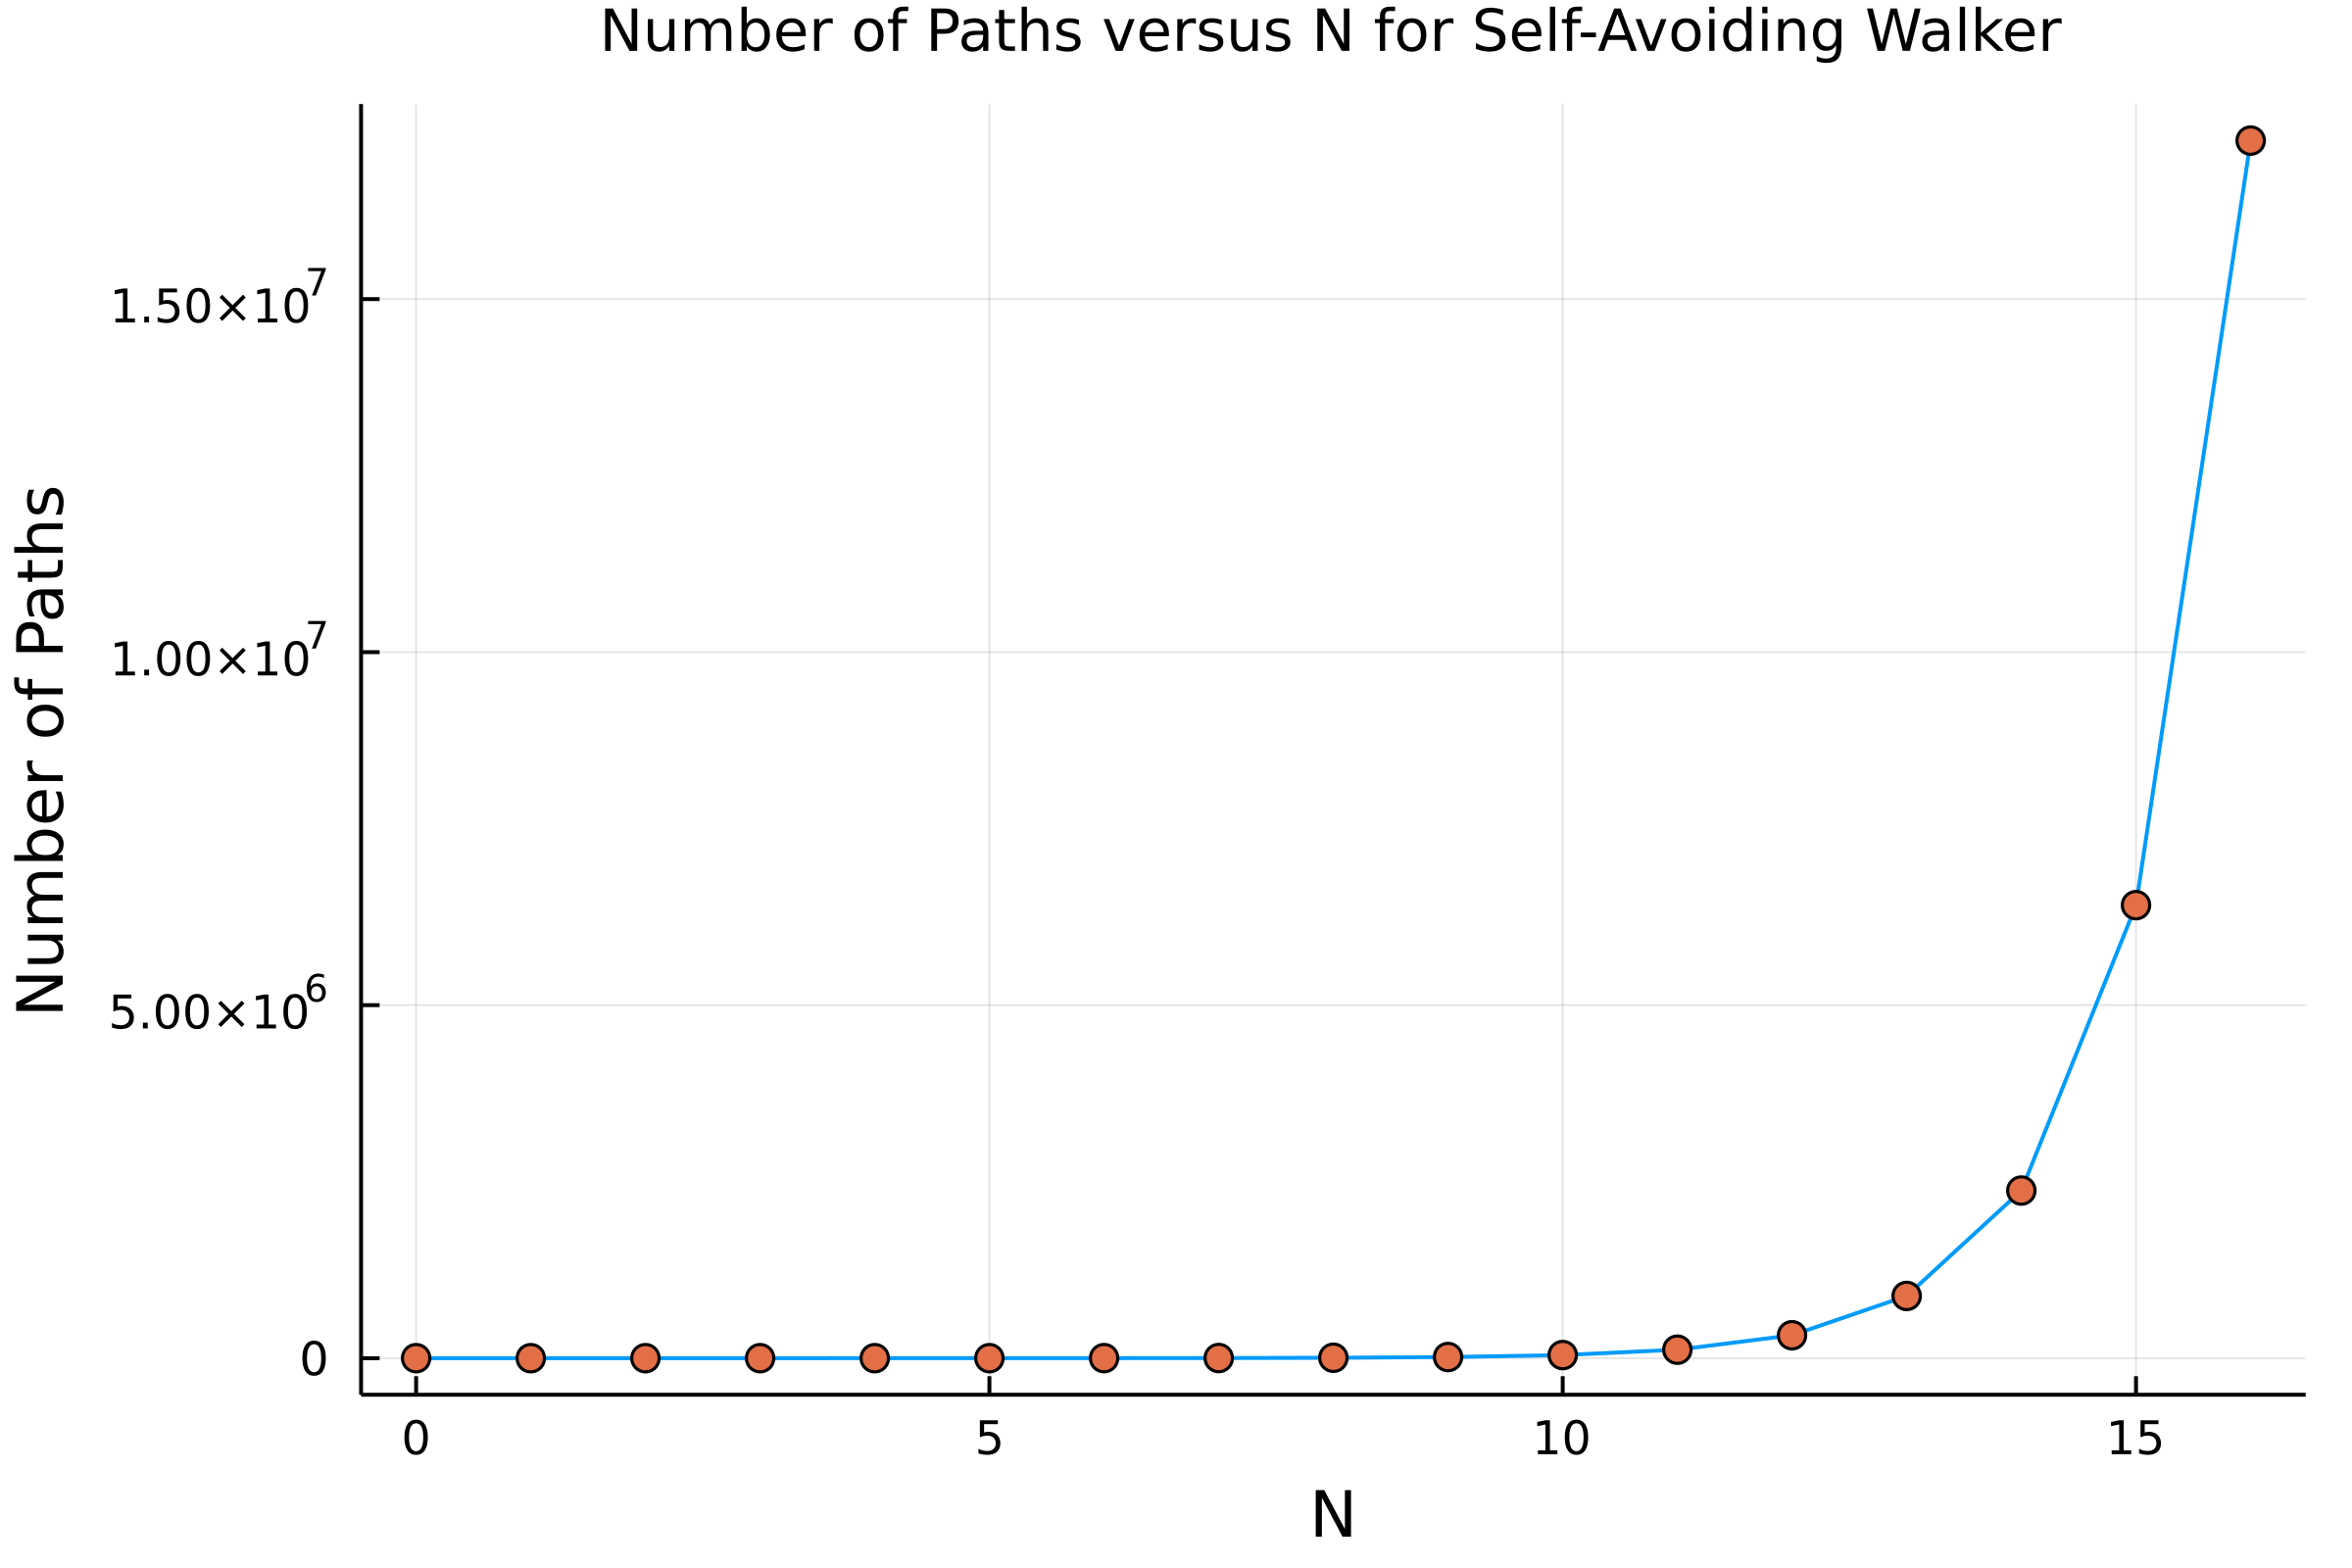
\includegraphics[width=\textwidth]{NumberOfPaths_N.png}
		\label{fig:mesh1.1}
		\caption{}
	\end{subfigure}\par\bigskip 
	\begin{subfigure}[t]{0.8\textwidth}
		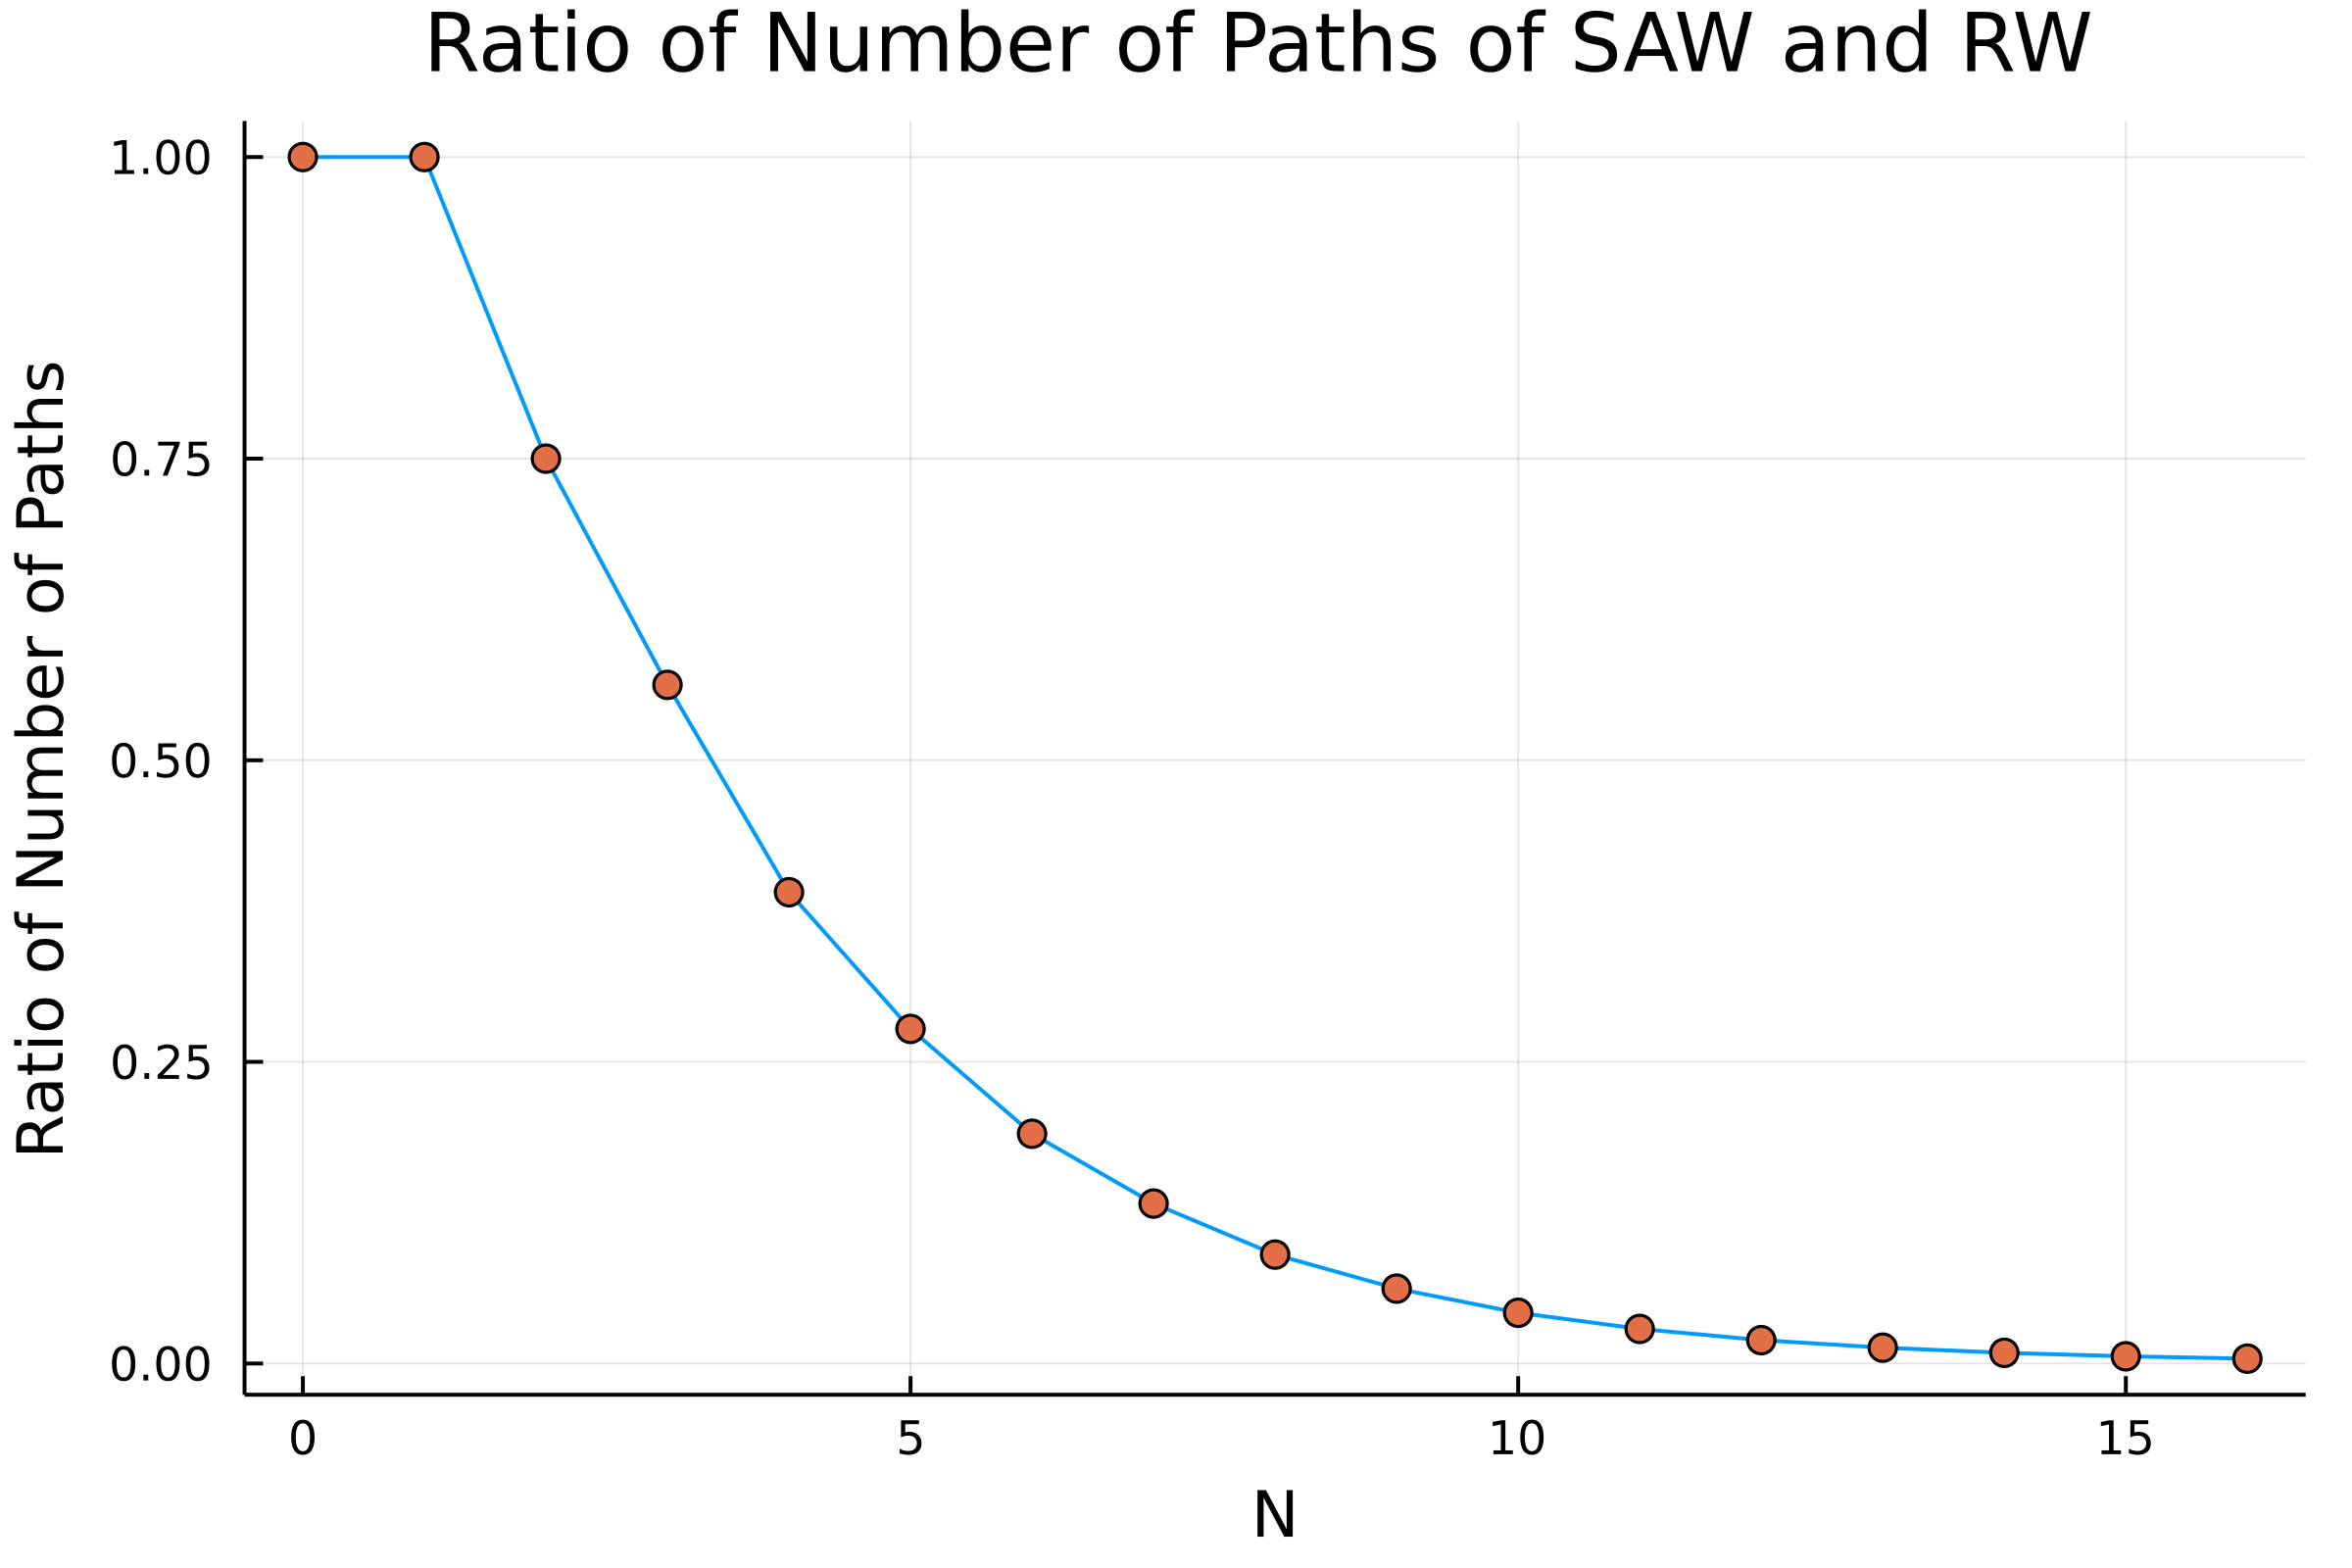
\includegraphics[width=\textwidth]{Ratio_N.png}
		\label{fig:mesh1.2}
		\caption{}
	\end{subfigure}
	\label{fig:mesh1}
	\caption{Figures wanted in example 4.7. N=16}
\end{figure}
\part*{4. Exercise 6.1: Generating Uniform Random Numbers}
\paragraph*{} It's clear from the Fig.3.a that according to our expectations, the amount of numbers generated for 0 $\leq$ digit $\leq$ 9 is about $\dfrac{1}{N}$. We intend to prove the following relation is acceptable:$\frac{\sigma}{N} \sim \frac{1}{\sqrt{N}} \rightarrow \log \sigma \sim \frac{1}{2} \log N$
\begin{figure}[H]
	\centering
	\begin{subfigure}[t]{0.8\textwidth}
		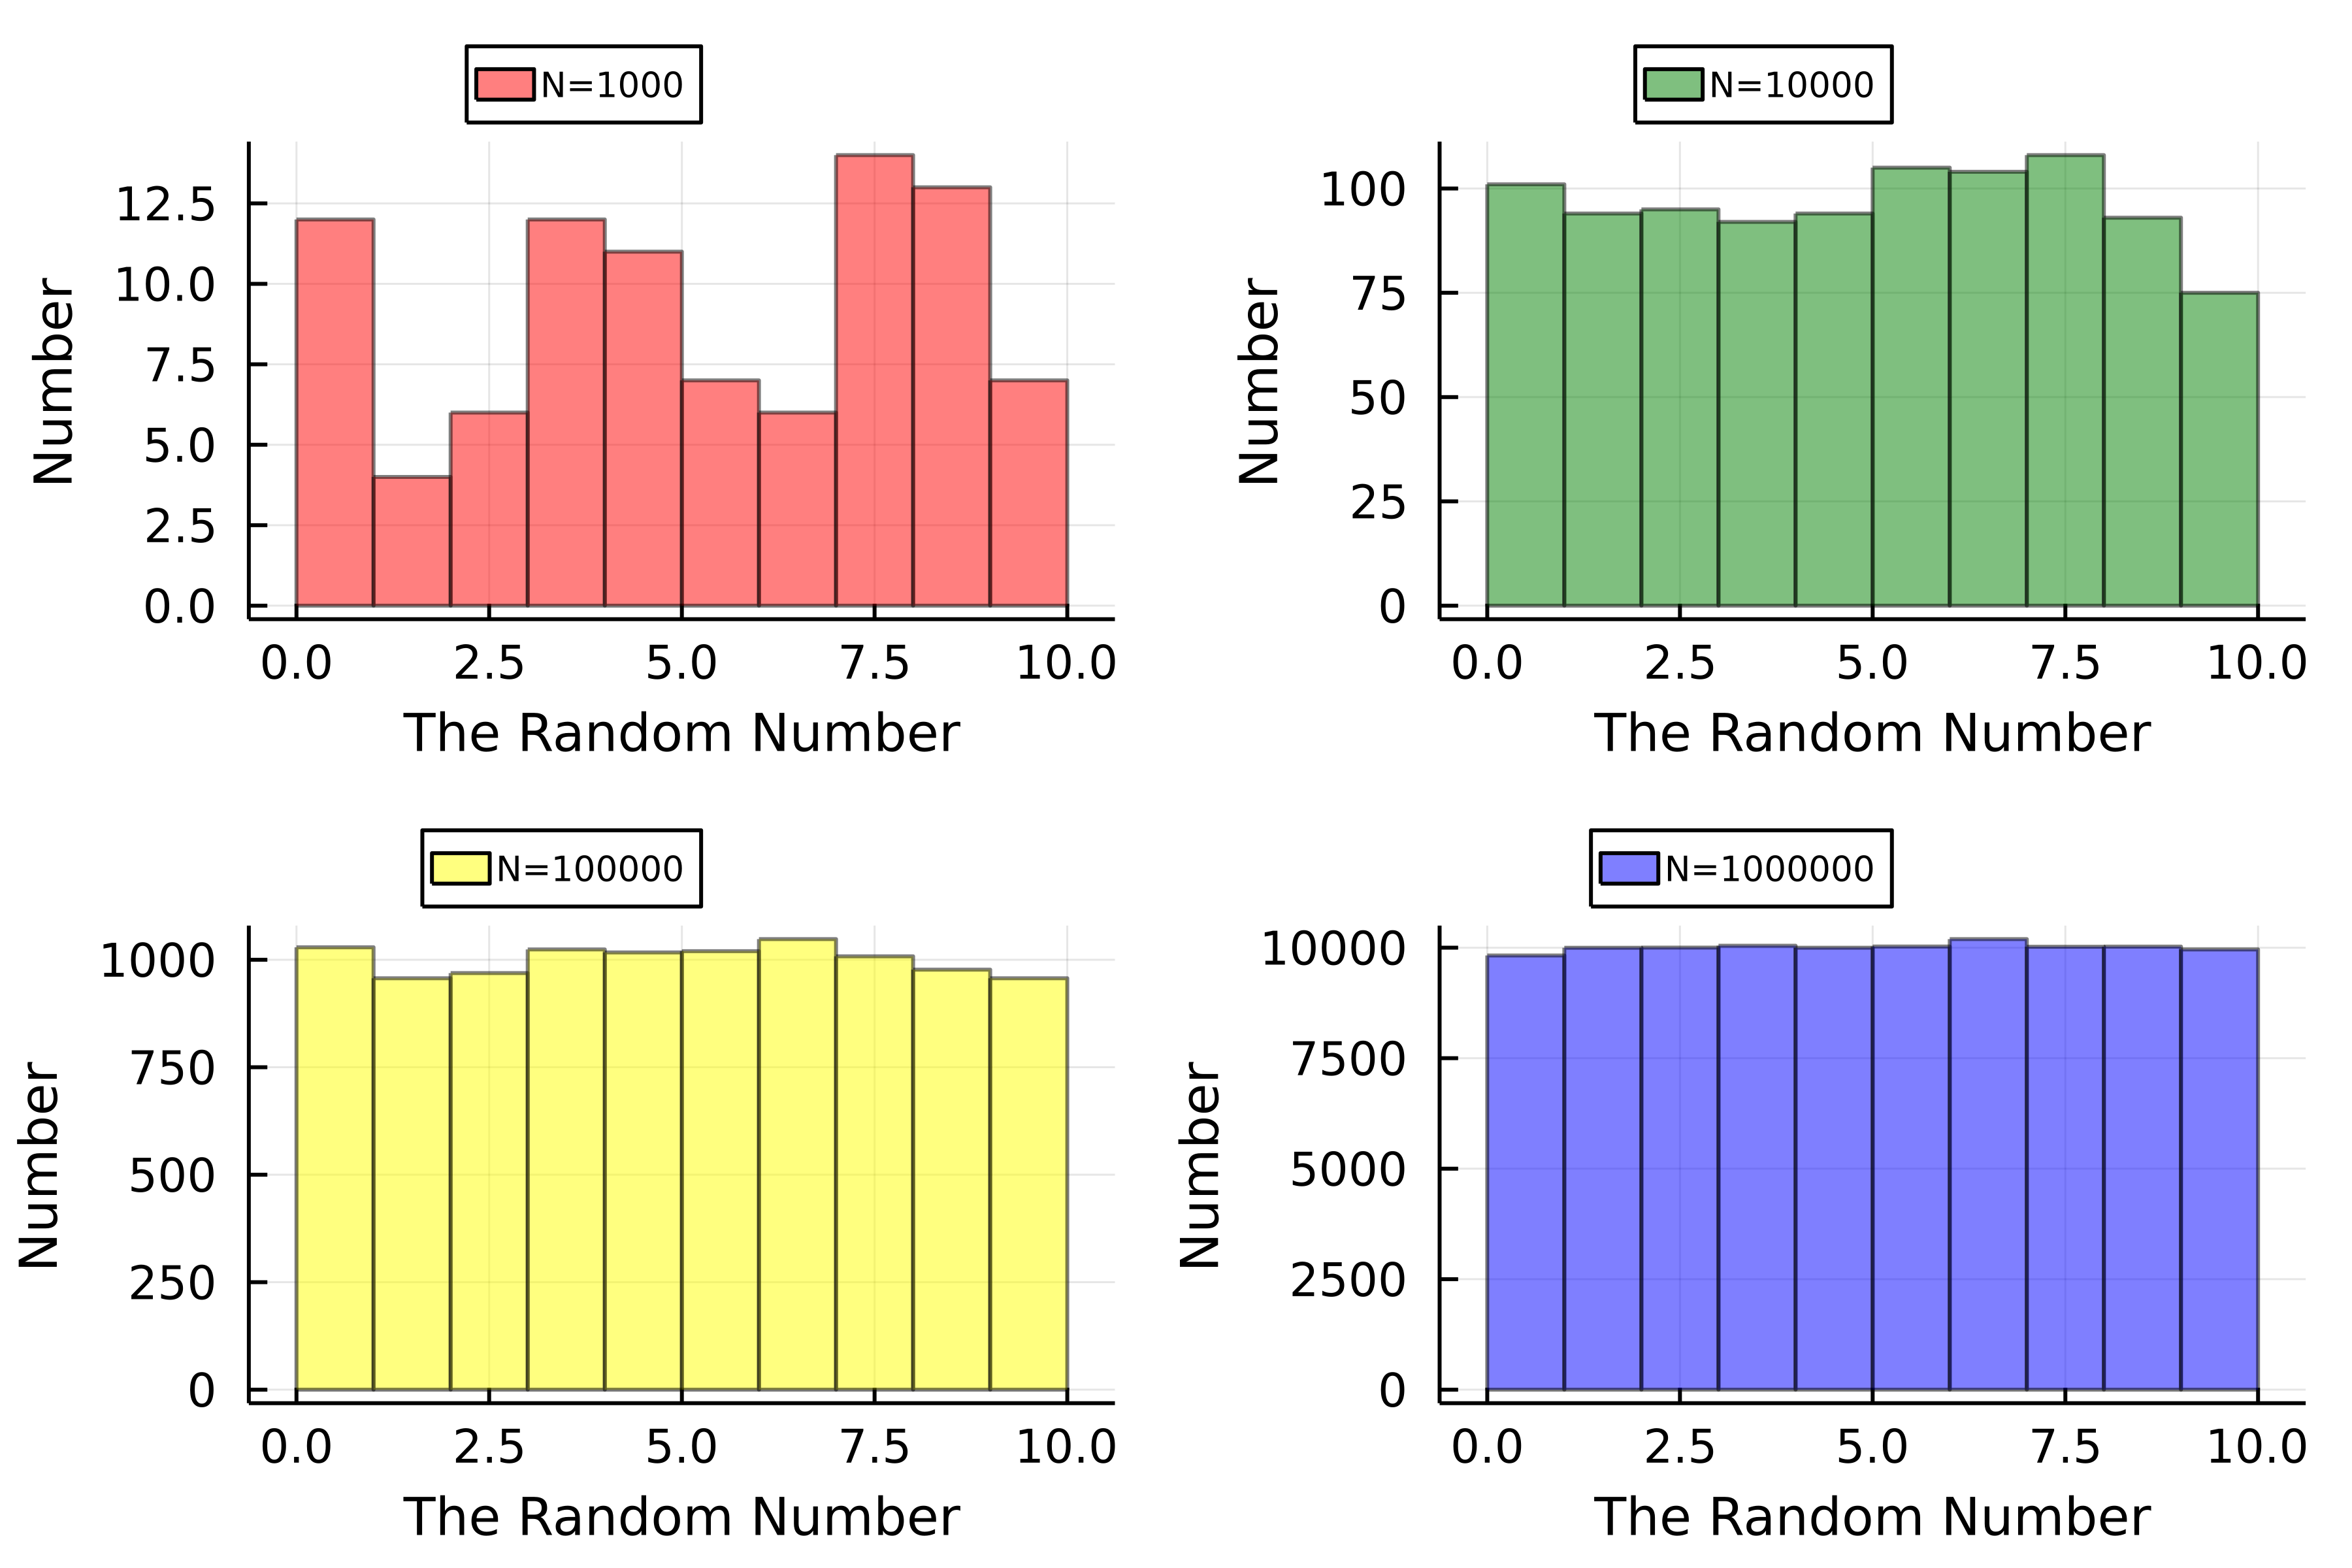
\includegraphics[width=\textwidth]{TheFrequencyCruve.png}
		\label{fig:mesh1.1}
		\caption{}
	\end{subfigure}\hfill%\par\bigskip 
	\begin{subfigure}[t]{0.48\textwidth}
		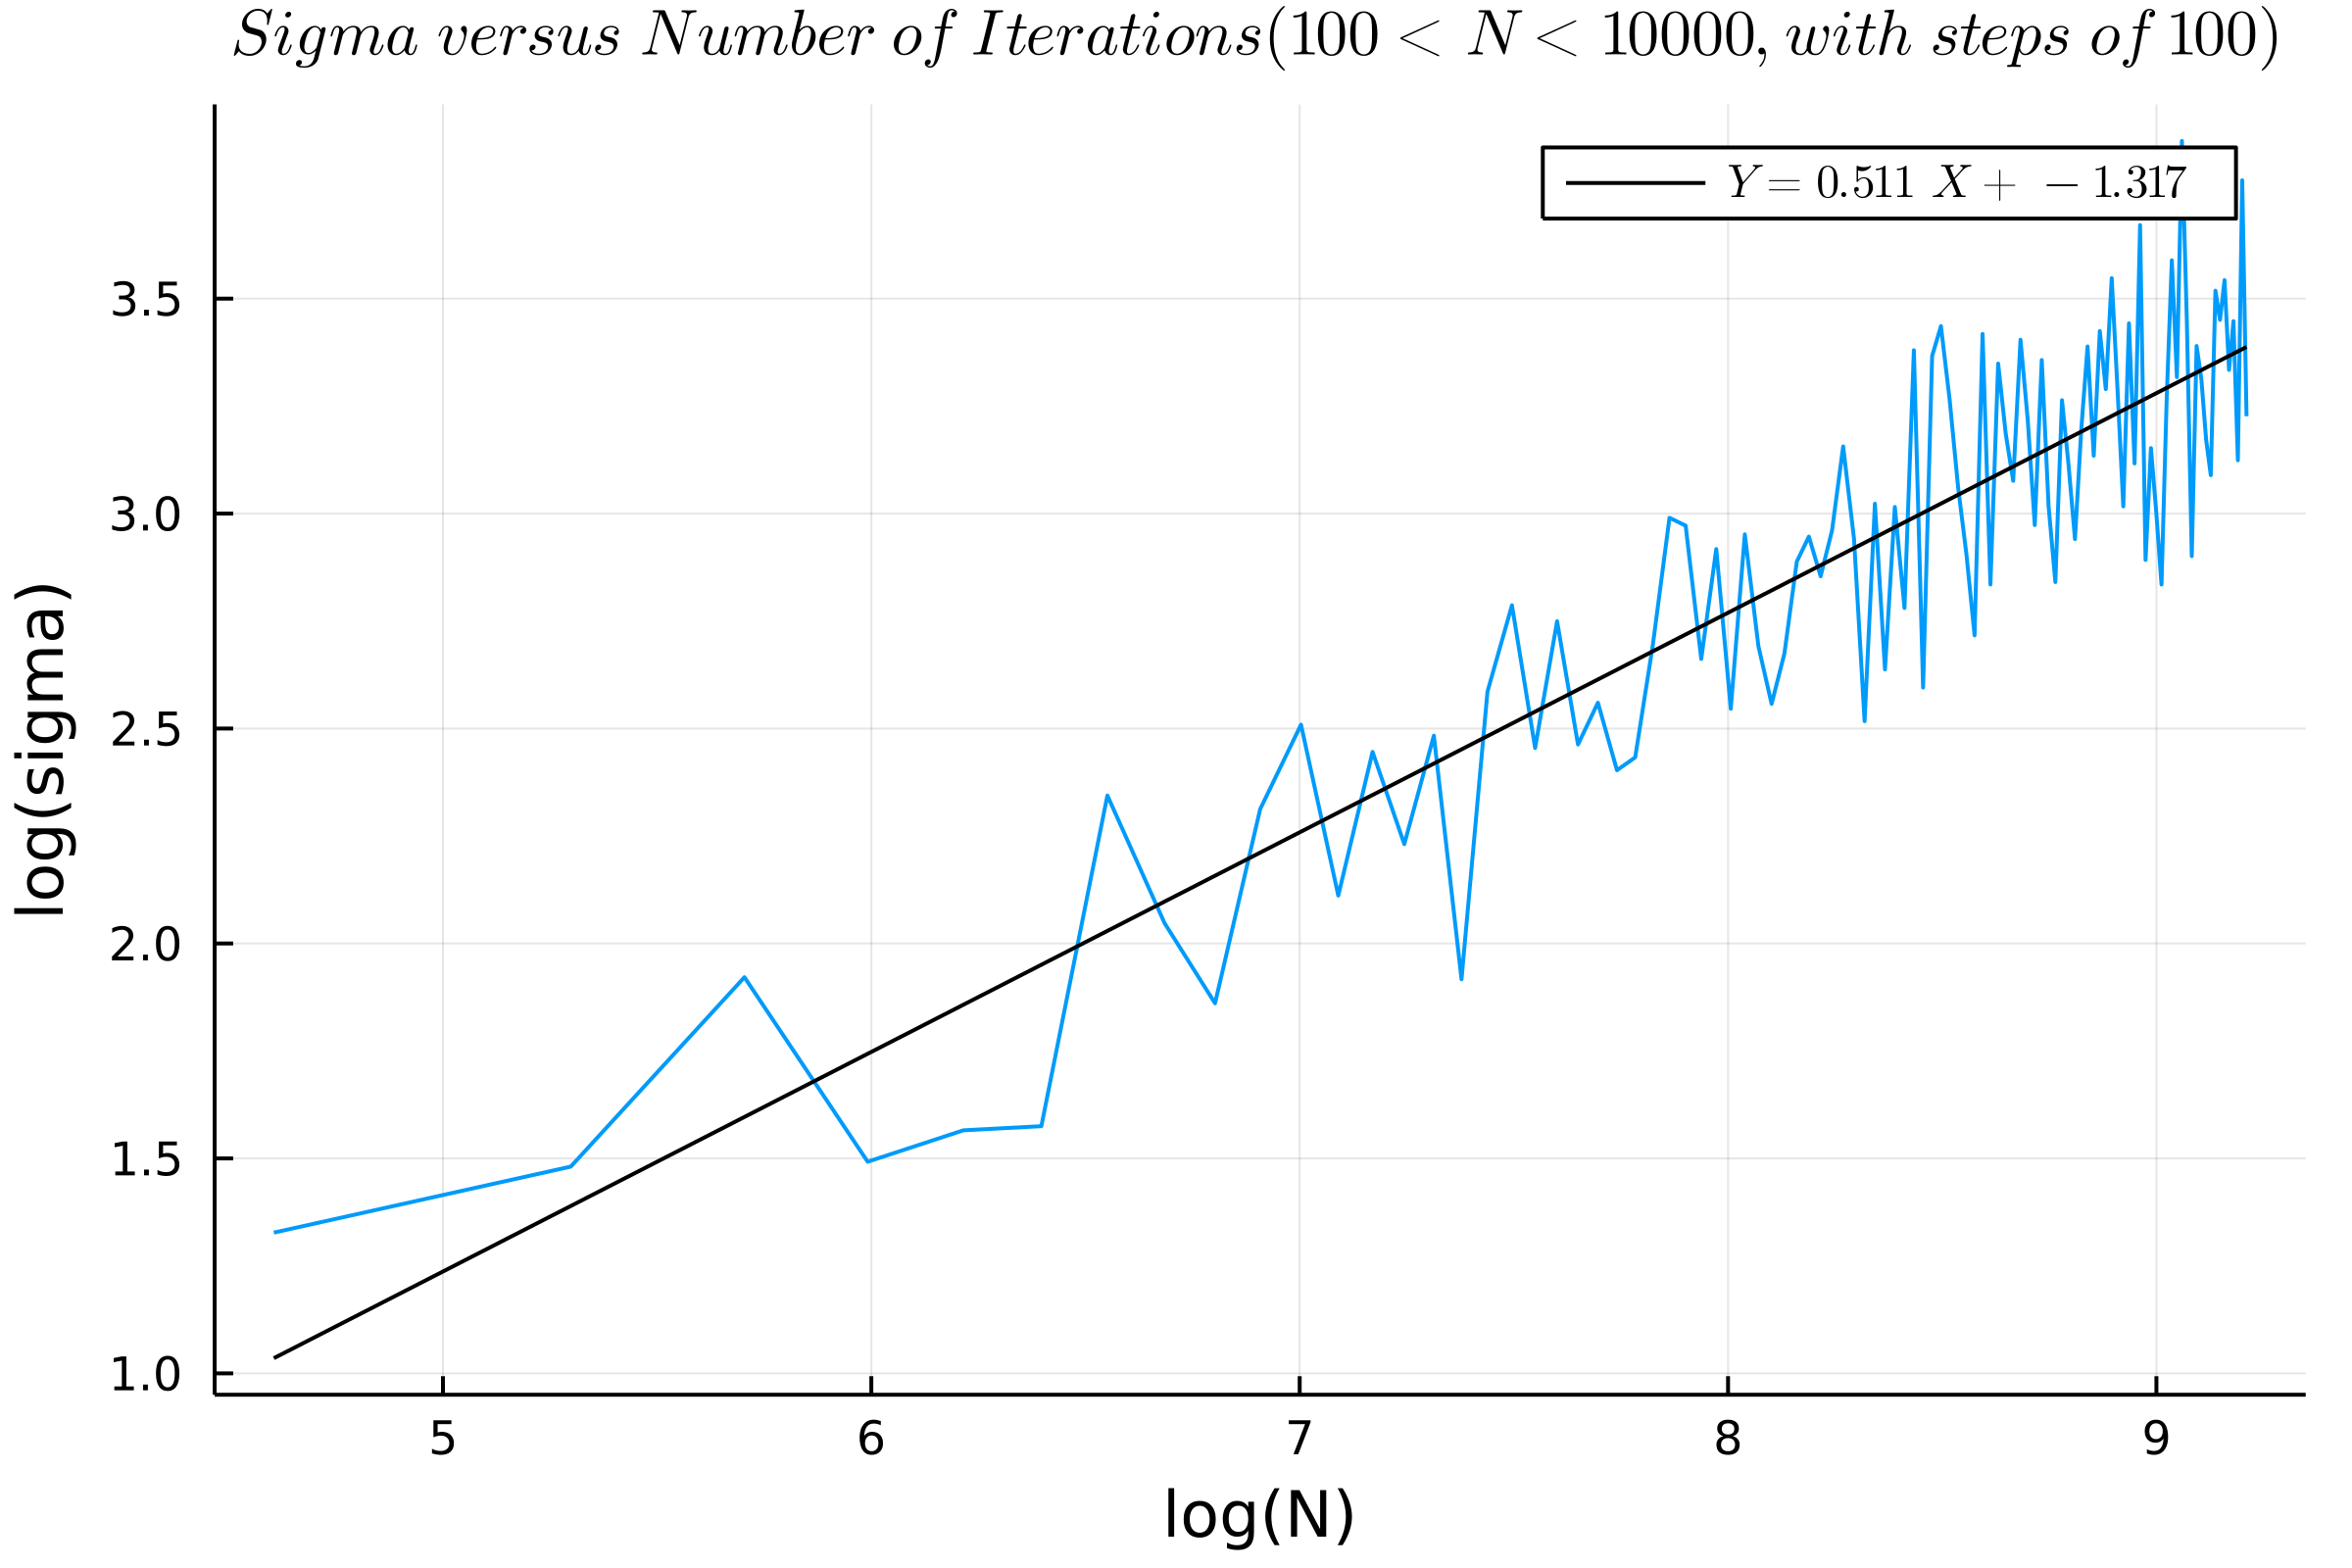
\includegraphics[width=\textwidth]{Sigma_N2.png}
		\label{fig:mesh1.2}
		\caption{}
	\end{subfigure}\hfill
	\begin{subfigure}[t]{0.48\textwidth}
		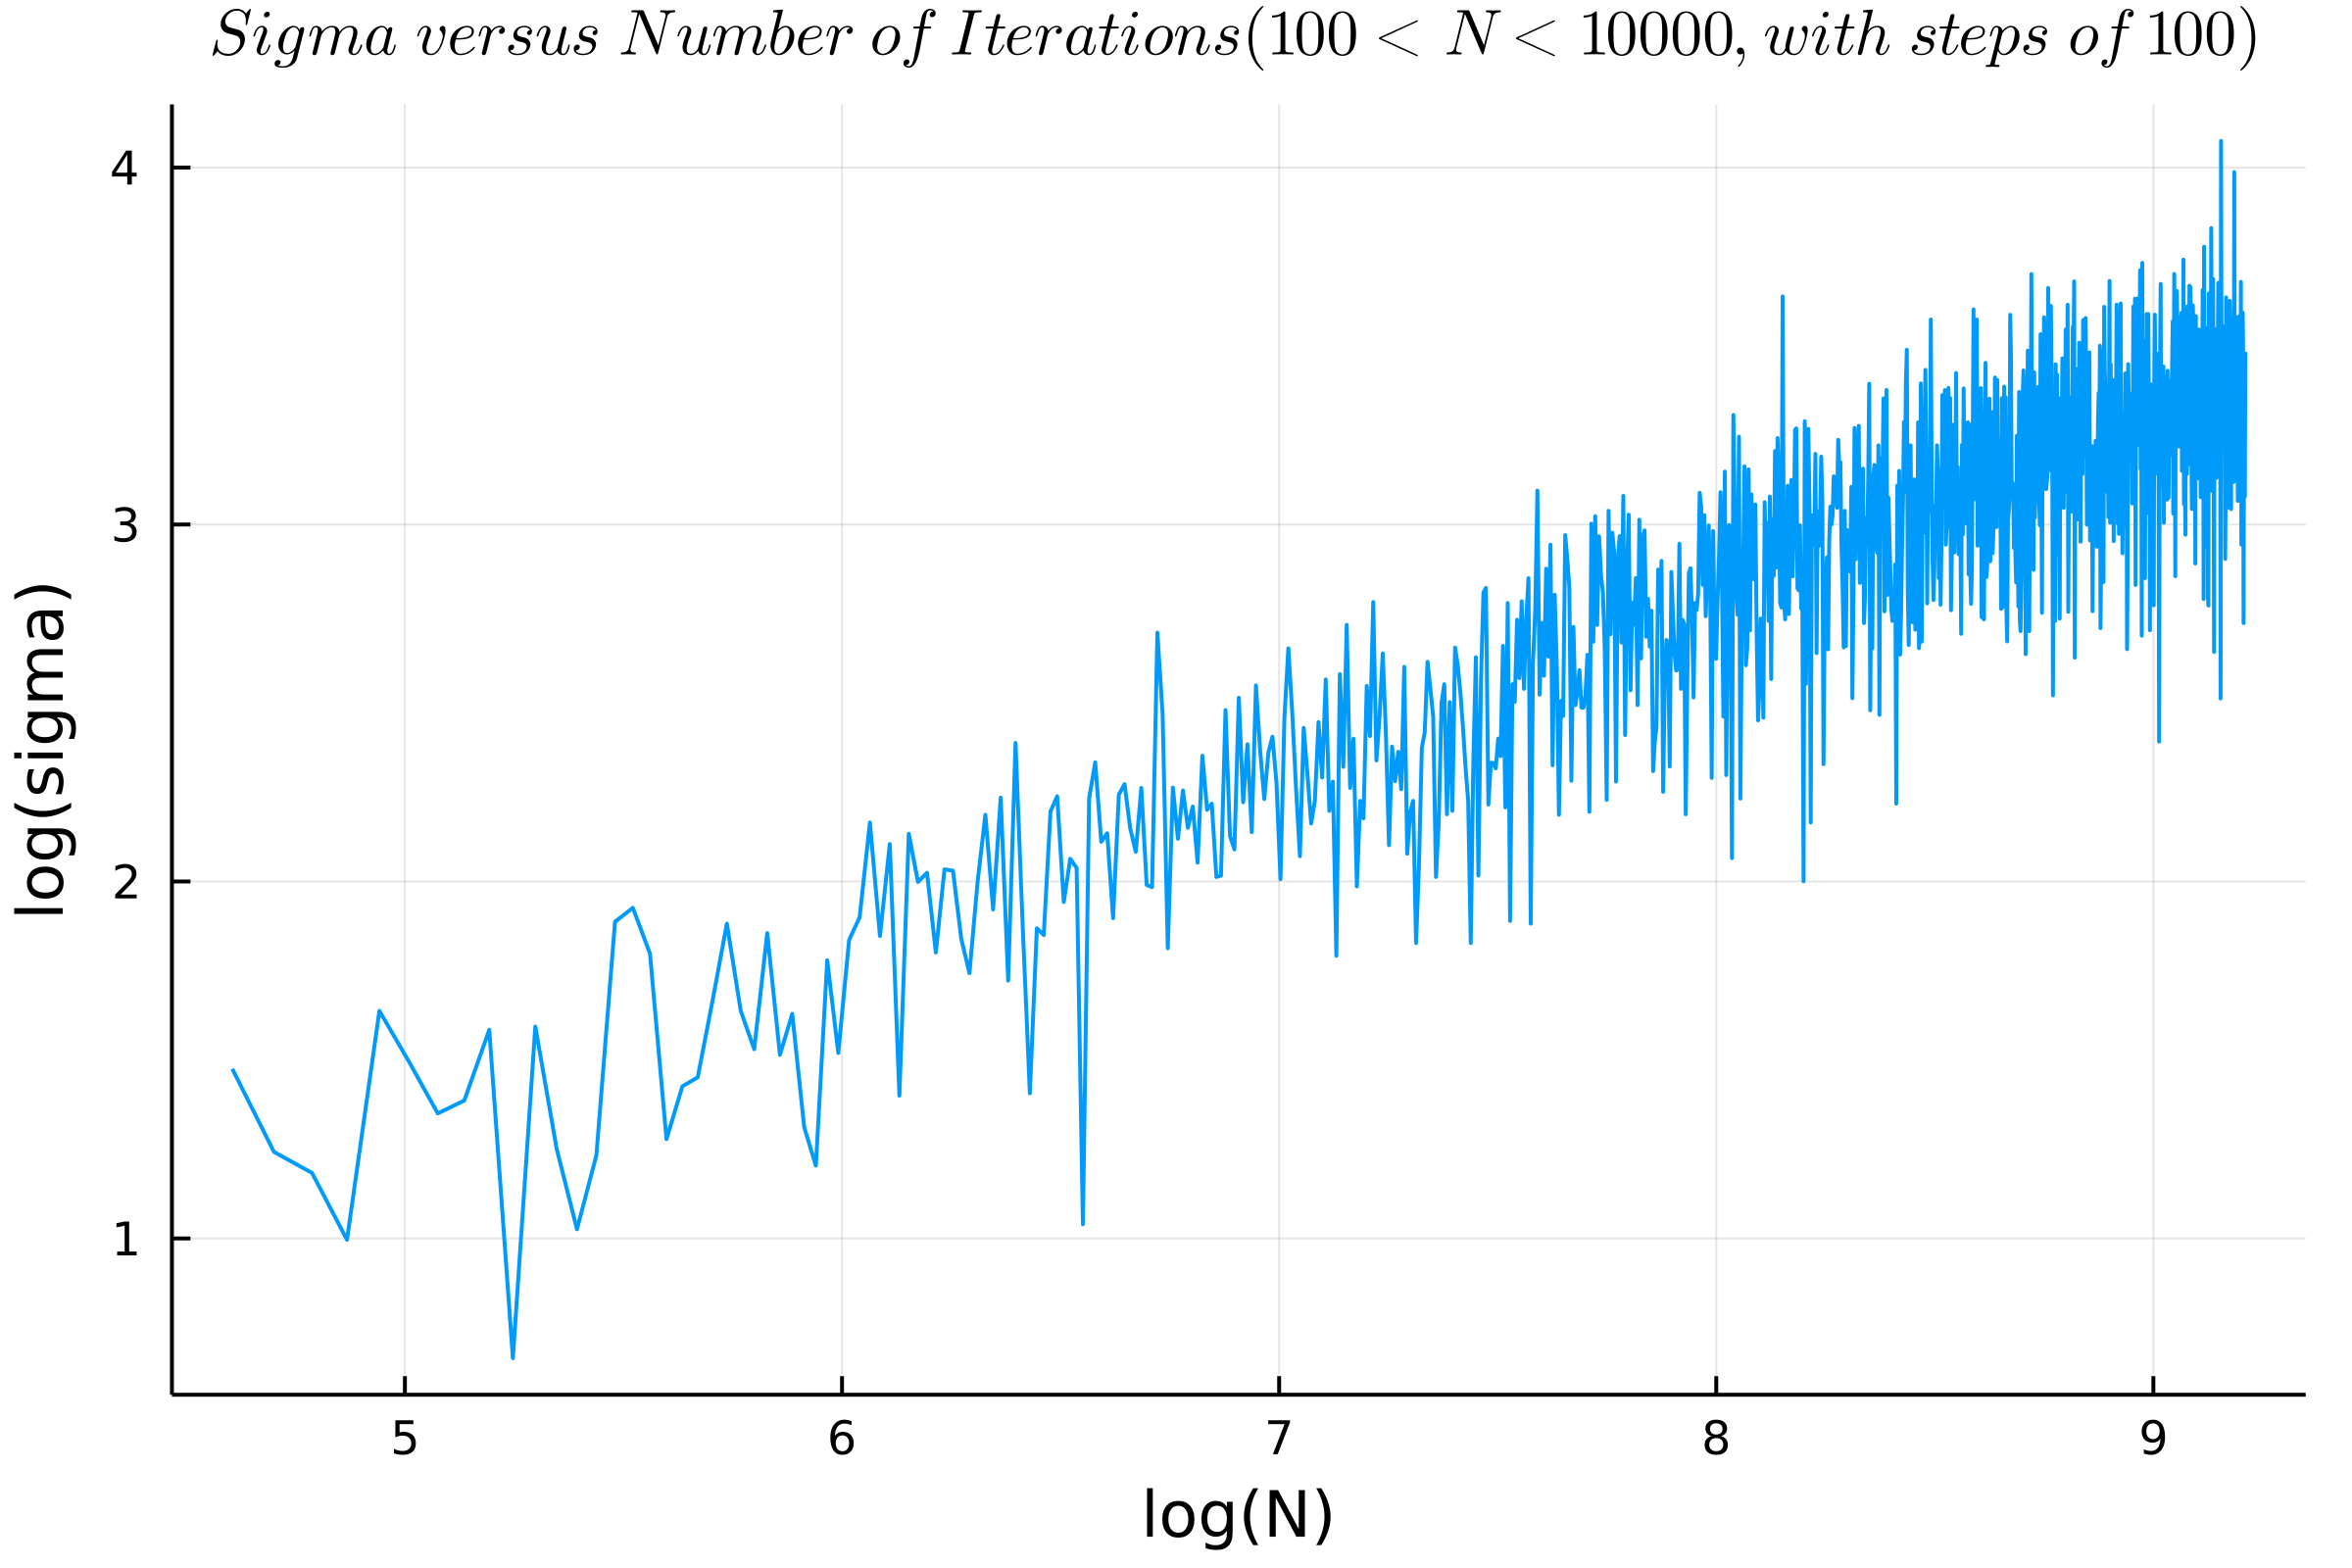
\includegraphics[width=\textwidth]{Sigma_N1.png}
		\label{fig:mesh1.2}
		\caption{}
	\end{subfigure}
	\label{fig:mesh1}
	\caption{Plots given for example 6.1. As you can see from the figures (a) and (b), the slopes of the plots are about 0.5, which confirms the relation above.}
\end{figure}
\part*{5. Exercise 6.2: Entanglement}
Doing what the exercise told, and found out that there are no entanglement. 
\begin{figure}[H]
	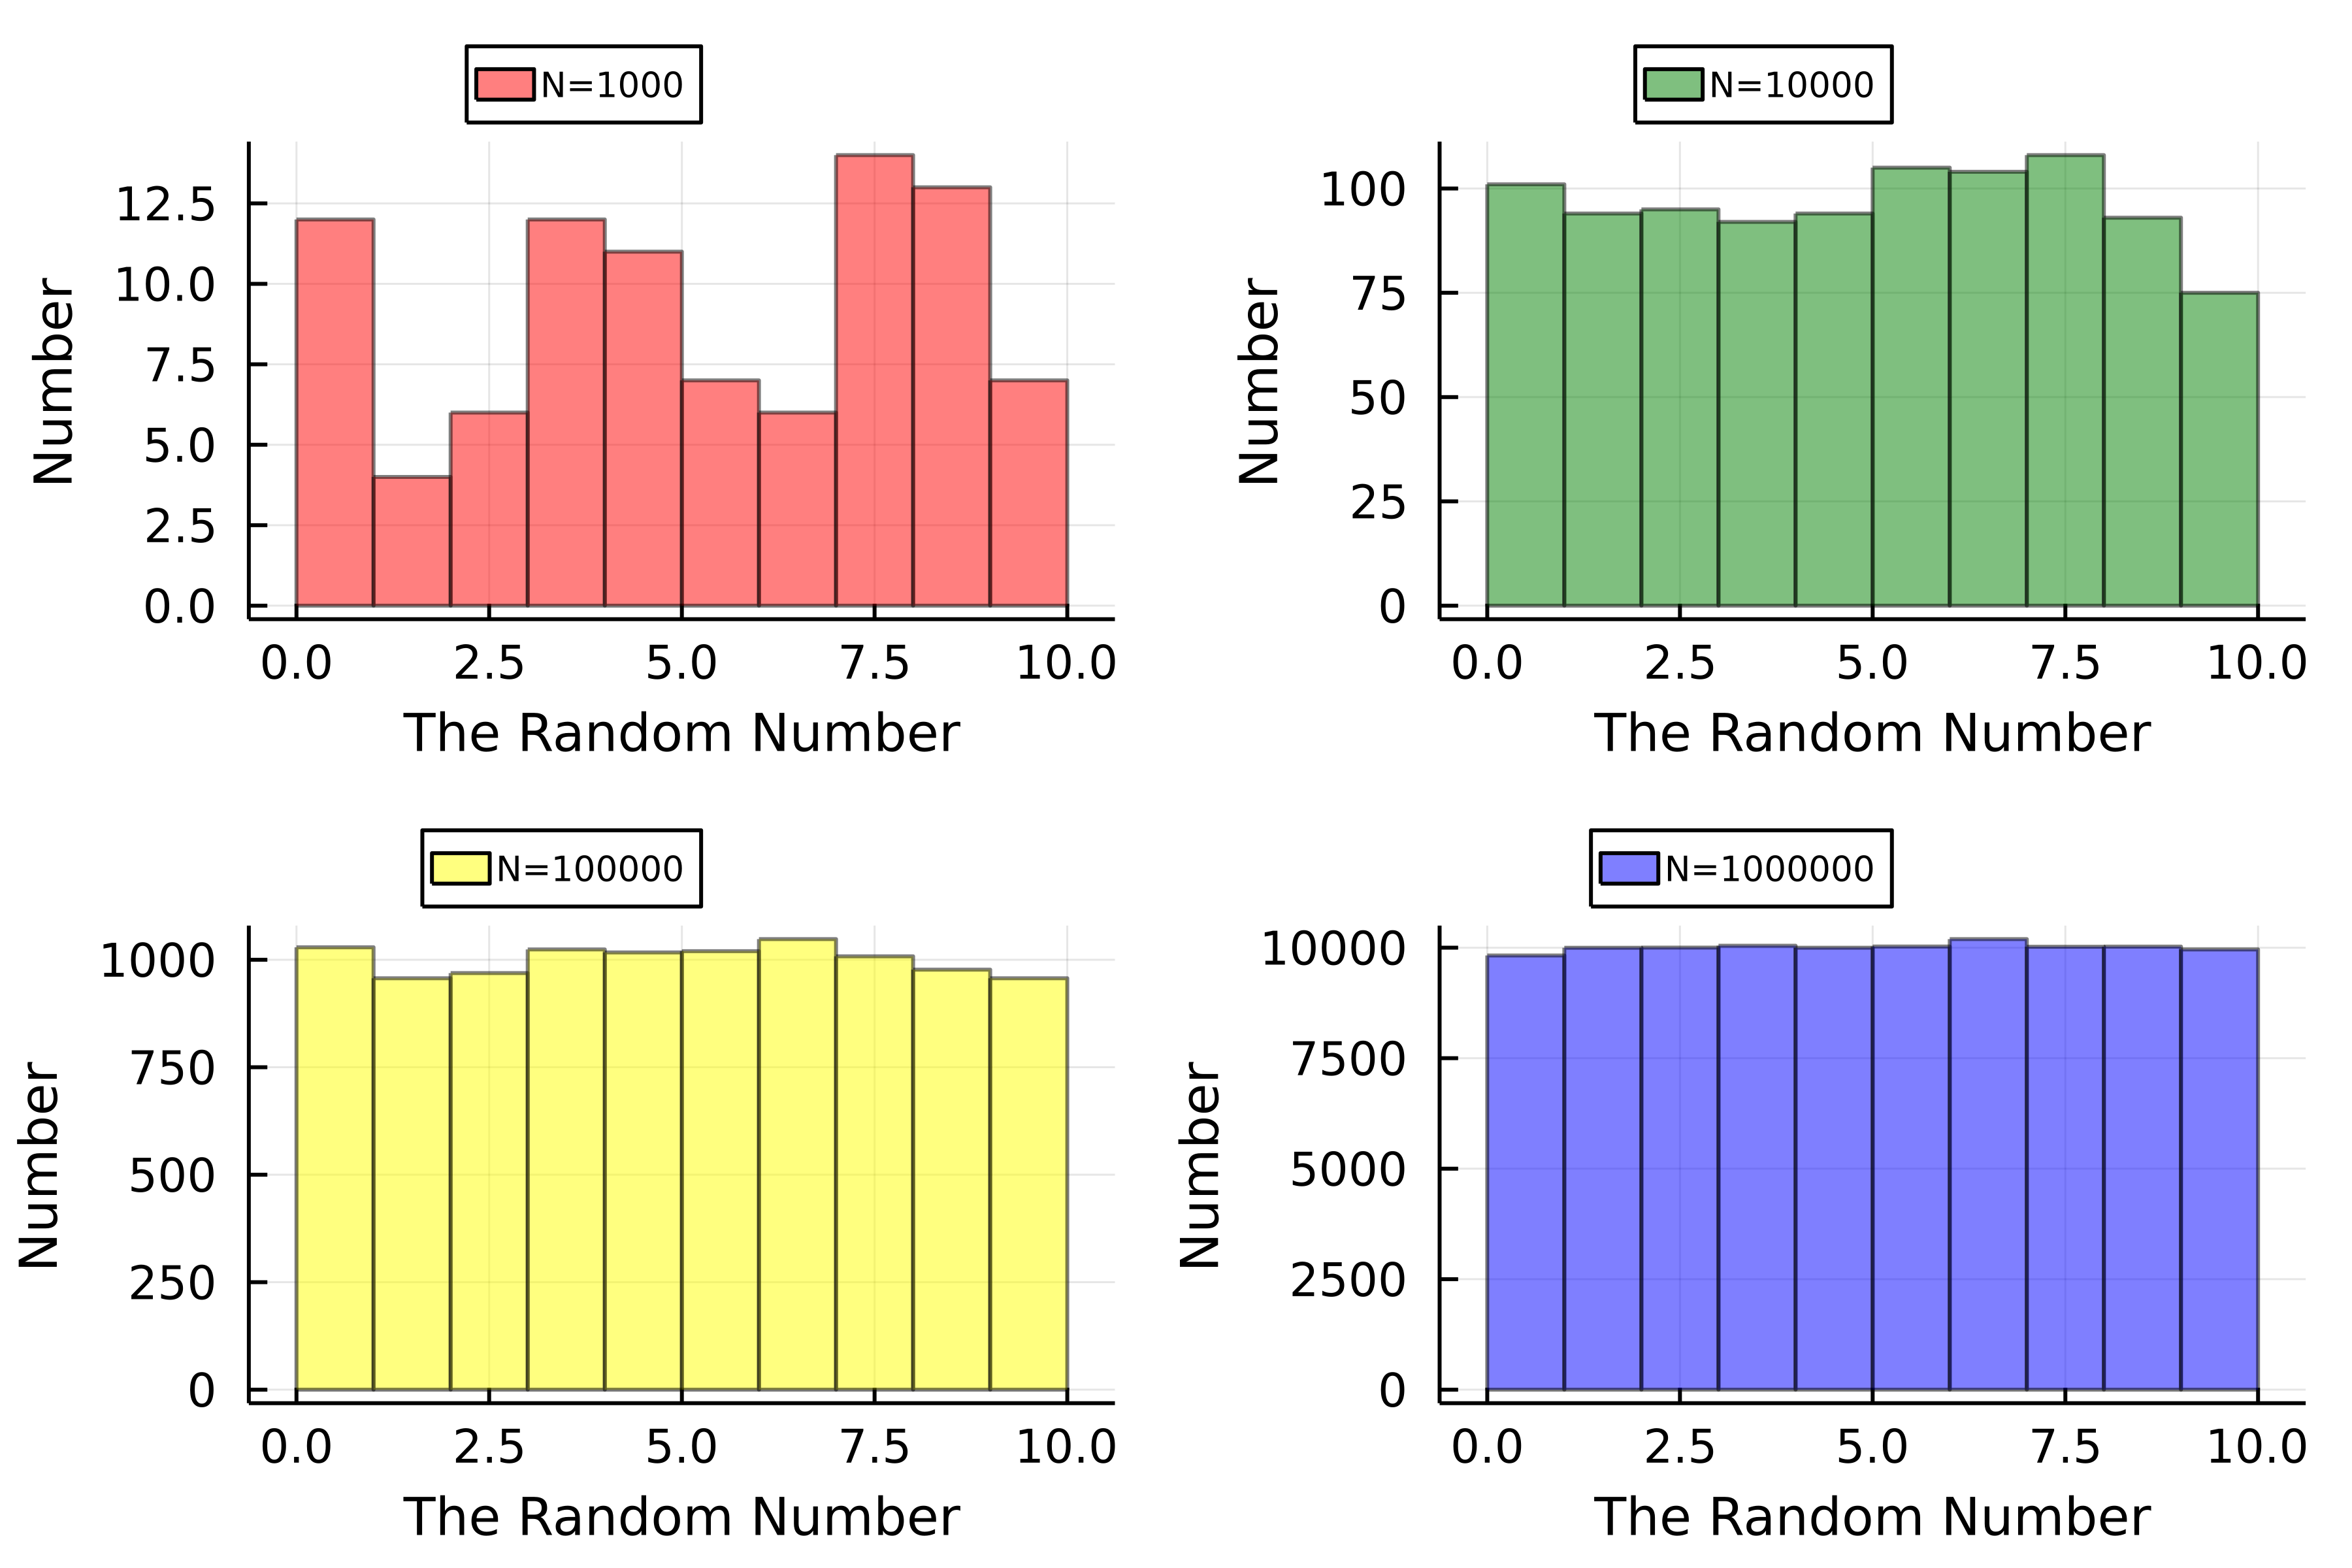
\includegraphics[width=\textwidth]{TheFrequencyCruve2.png}
	\label{fig:mesh4}
	\caption{Figures confirming the uniform distribution function for exercise 6.2.}
\end{figure}
\end{document}